\documentclass{beamer}

%%%%%%%%%%%%%Solarized Theme%%%%%%%%%%%%%%%
\usecolortheme[dark,accent=cyan]{solarized}
\beamertemplatenavigationsymbolsempty

%%%%%Packages%%%%%
\usepackage{graphicx}
\usepackage{hyperref}
\usepackage{colortbl, xcolor}
\usepackage{booktabs}
\usepackage{standalone}
\usepackage{tikz}
\usetikzlibrary{positioning, arrows, calc, shapes.arrows}

\usepackage{minted}

\definecolor{DarkGray}{gray}{0.1}
\definecolor{DarkGray}{gray}{0.1}
\usemintedstyle{native}

%%%%%%Title%%%%%%%%
\title{Rhinos with a bit of Python}
\author{@NikoletaGlyn}
\date{ \small{Tamsin E. \textsc{Lee} \hspace{1cm} Vincent \textsc{Knight}}}
\institute[]
{
\begin{center}
    
\includegraphics[width=.15\textwidth]{static/cardiff_uni_logo.jpg}\hspace{.5cm}
    
\includegraphics[width=.153\textwidth]{static/pycon-namibia.png}
\end{center}
}

\begin{document}

\maketitle  

\begin{frame}
	\begin{center}
		\Huge \textbf{\textcolor{orange}{rhino-ceros}}
	\end{center}
\end{frame}

\begin{frame}
	\begin{center}
    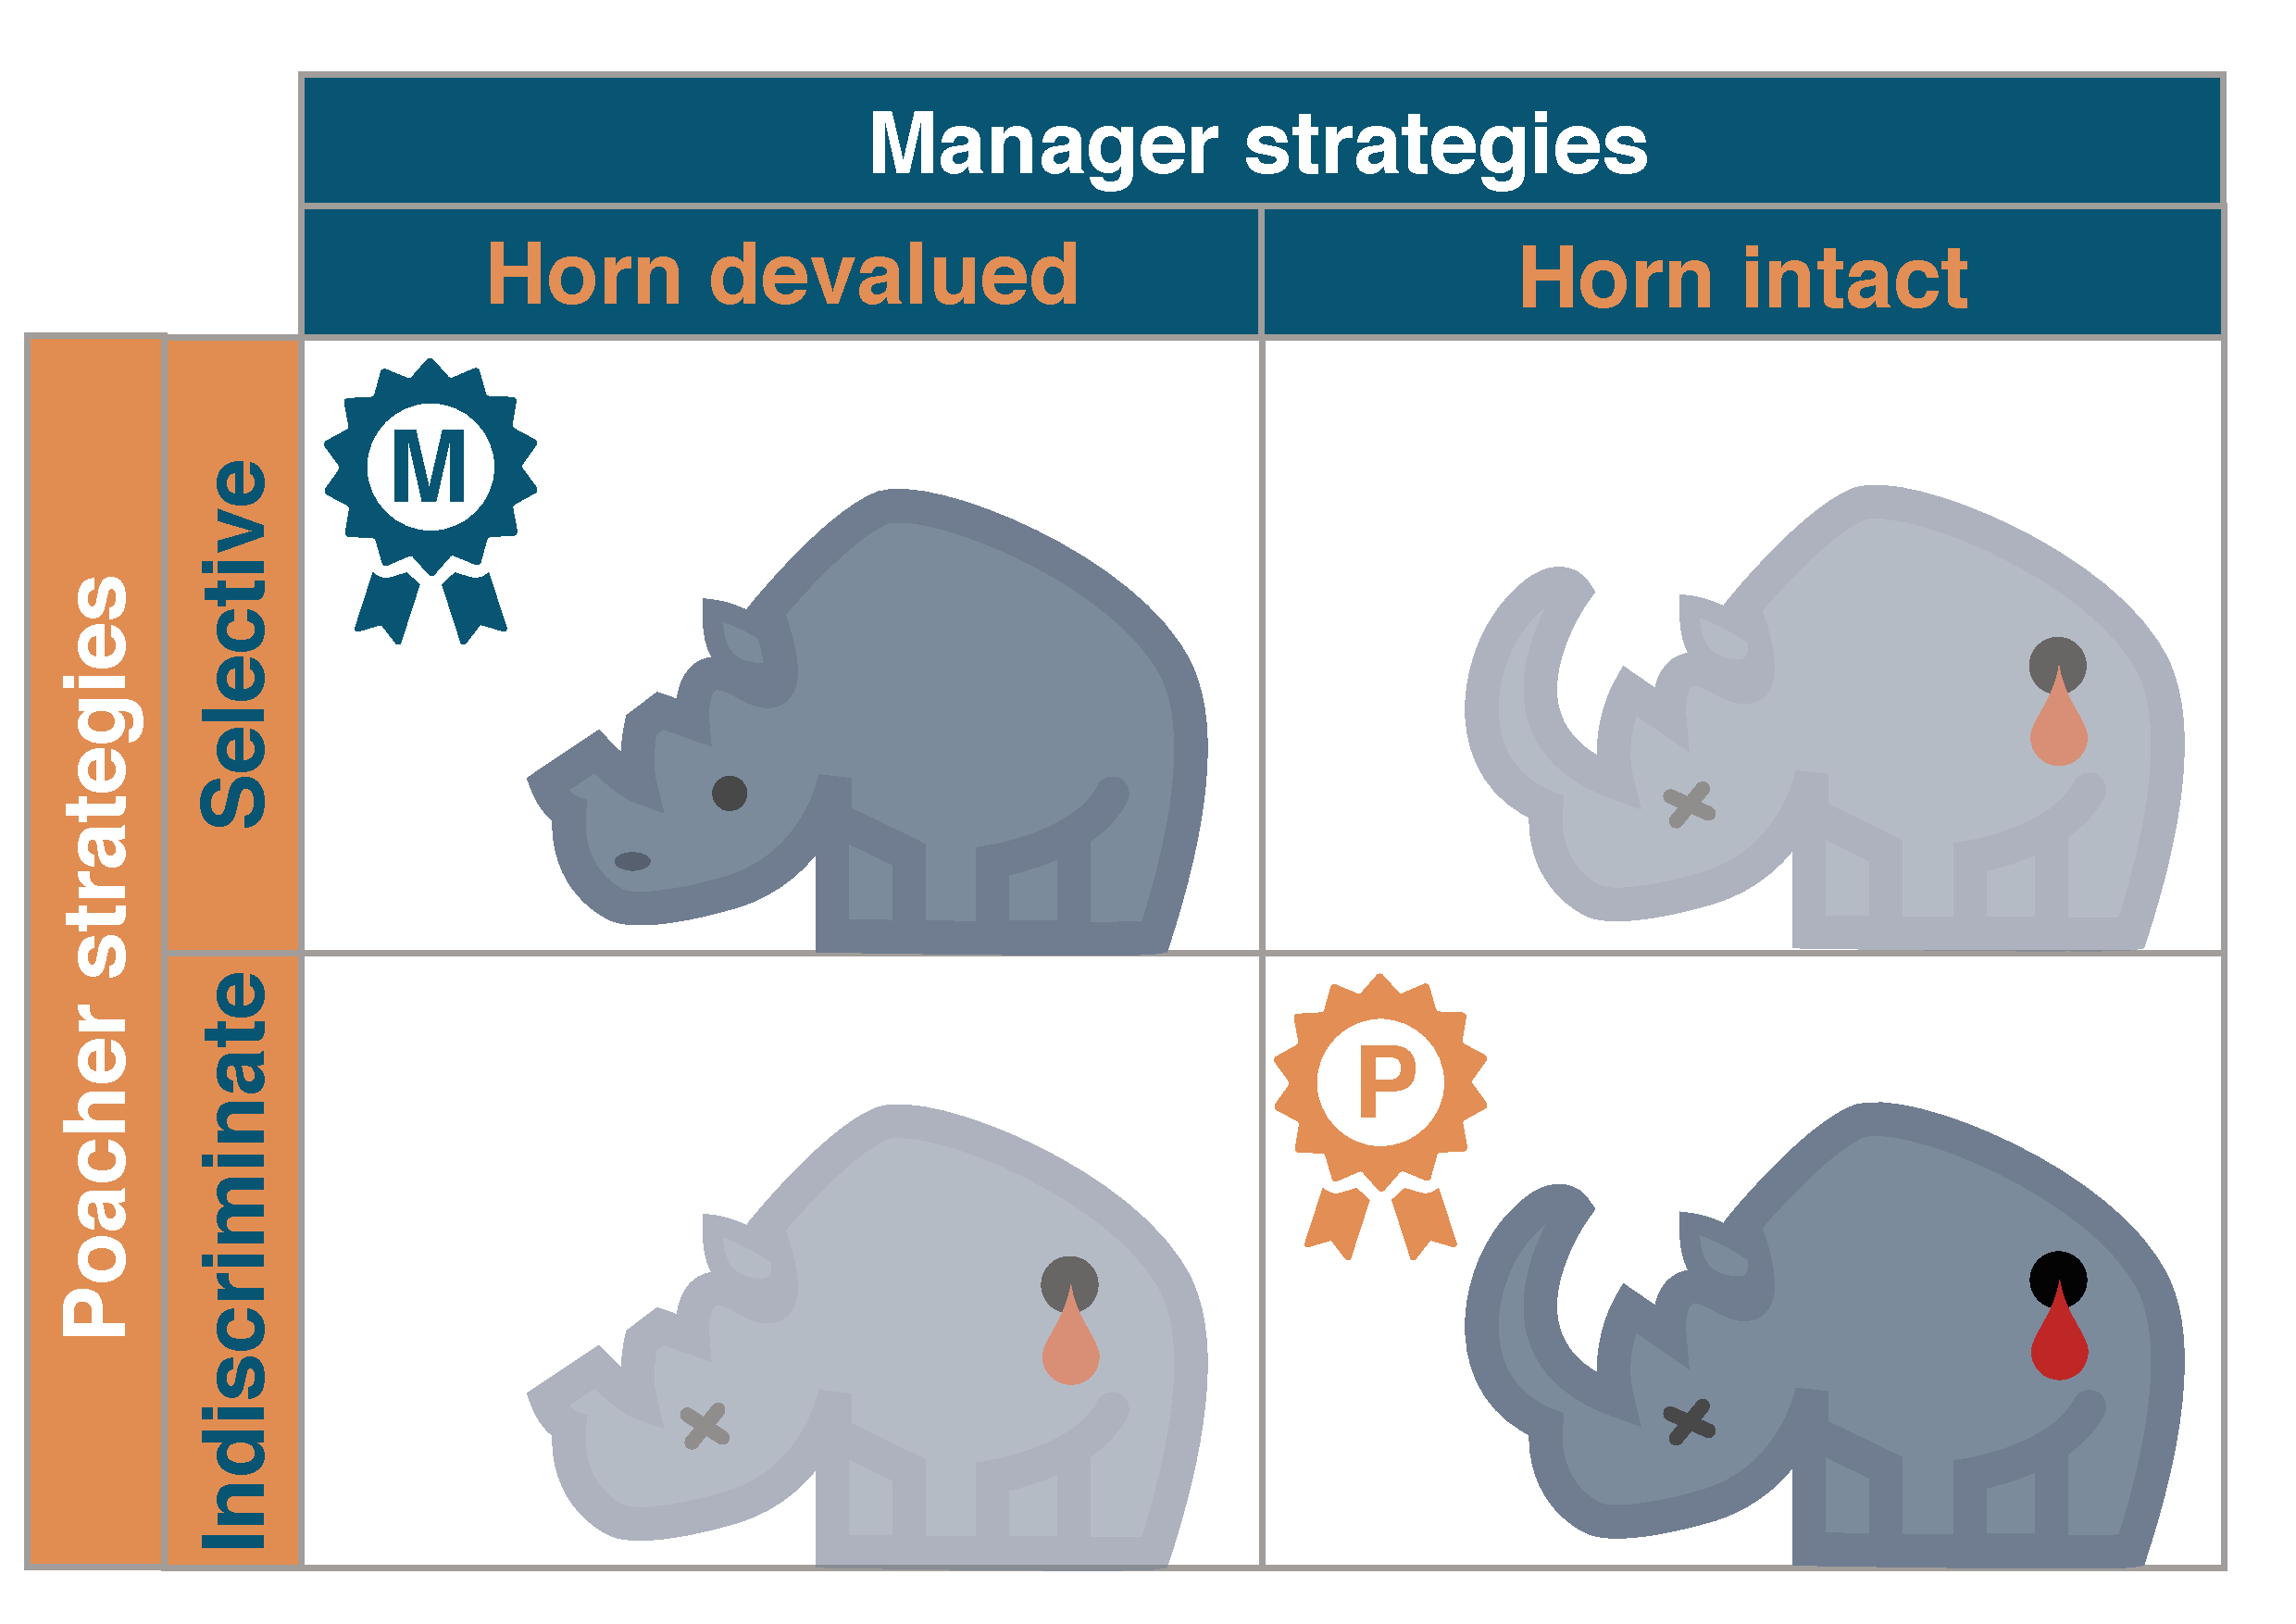
\includegraphics[width=\textwidth]{static/RhinoPic.pdf}

    \footnotesize{\textcolor{orange}{\textbf{Devaluing rhino horns as a theoretical game. Tamsin E. Lee, David L. Roberts.} 2016}}
	\end{center}
\end{frame}

\begin{frame}
    \begin{center}
    \includestandalone[width=\textwidth]{static/poachers}
    \end{center}
\end{frame}

\begin{frame}
    \begin{center}
    \includestandalone[width=\textwidth]{static/evolutionary_study}
    \end{center}
\end{frame}

\begin{frame}
    \begin{center}
    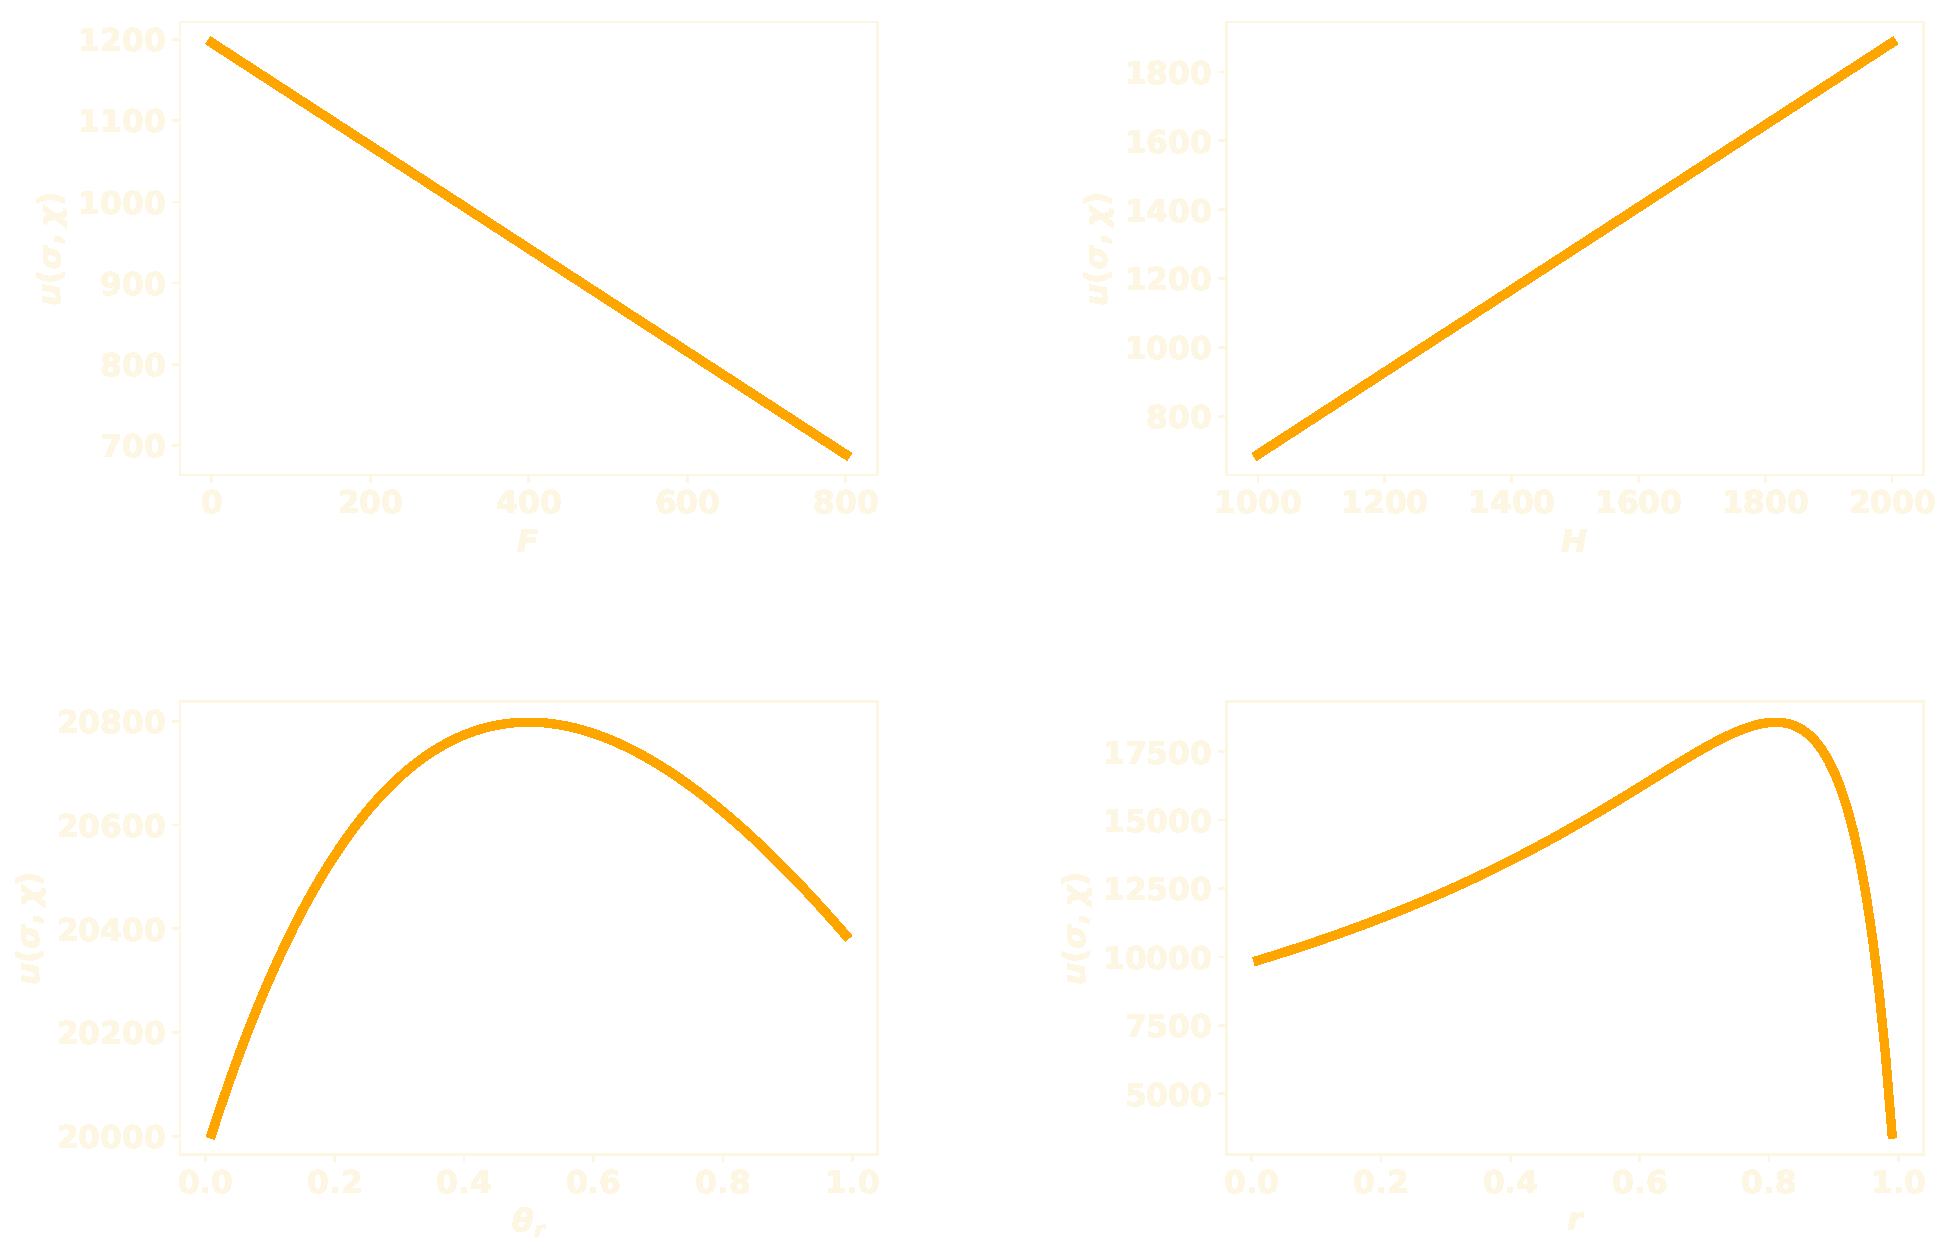
\includegraphics[width=.8\textwidth]{static/utility}
    \end{center}
\end{frame}

\begin{frame}
    \centering
    \large{
    \textcolor{orange}{
        \rotatebox{-35}{
            \(\mathbf{u(\sigma, \chi)} = \mathbf{H (\theta_r r(1 - s) - r + 1) \theta(r, x)^{-\alpha} -}
            \mathbf{F \left(1 - s + \frac{s}{1 - r} \right)(1-rx)^{\gamma}(1 - r)^{\beta}}\)
    }}}
    \end{frame}

\begin{frame}
    \begin{center}
    \includestandalone[width=\textwidth]{static/evolutionary_study}
    \end{center}
\end{frame}
    
\begin{frame}
    \centering
    \footnotesize
    \begin{theorem}[Selective]
    A population of selective poachers is unstable.
    \end{theorem}

    \begin{proof}
    \[u(1, 1)  > u(0, 1),\]
    where
    \[u(1, 1) = H(1 - r)^{1 - \alpha} − F (1 - r)^{\beta + \gamma - 1}\]
    and
    \[u(0, 1) = H(\theta_{r} r + 1 - r)(1 - r)^{-\alpha} - F (1 - r)^{\beta + \gamma}.\]
    This gives the condition,
    \[H\theta_{r} < -F (1 - r)^{\gamma + \beta + \alpha -1}\]
    \end{proof}
\end{frame}

\begin{frame}[fragile]
	\begin{minted}
    [
    framesep=4mm,
    baselinestretch=1.2,
    bgcolor=DarkGray,
    fontsize=\footnotesize,
    ]
    {python}
>>> import sympy as sym
    \end{minted}
\vspace{.5cm}
\pause
	\begin{minted}
        [
        framesep=4mm,
        baselinestretch=1.2,
        bgcolor=DarkGray,
        fontsize=\footnotesize,
        ]
        {python}
>>> (2 + 3) ** 2
25
\end{minted}
\vspace{.5cm}
\pause
\begin{minted}
    [
    framesep=4mm,
    baselinestretch=1.2,
    bgcolor=DarkGray,
    fontsize=\footnotesize,
    ]
    {python}
>>> a, b = sym.symbols('a, b')
>>> expr = (a + b) ** 2
>>> expr.expand()
a**2 + 2*a*b + b**2
    \end{minted}
\end{frame}

\begin{frame}[fragile]
	\begin{minted}
    [
    framesep=4mm,
    baselinestretch=1.2,
    bgcolor=DarkGray,
    fontsize=\tiny,
    ]
    {python}
>>> import imp
>>> tools = imp.load_source('tools', '../tools.py')

>>> tools.utility(1, 1)
-F*(-r + 1)**beta*(-r + 1)**gamma/(-r + 1) + H*(-r + 1)*(-r + 1)**(-alpha)

>>> tools.utility(0, 1)
-F*(-r + 1)**beta*(-r + 1)**gamma + H*(-r + 1)**(-alpha)*(r*(theta_r - 1) + 1)
    \end{minted}
\end{frame}


\begin{frame}
    \centering
    \footnotesize
    \begin{theorem}[Mixed]
        A mixed stable strategy \((s = s^{\star})\) never exists for \(0 < r < 1\).
    \end{theorem}

    \pause
    \vspace{1cm}
    \centering
    \footnotesize
    \begin{theorem}[Indiscriminate]
        A population of indiscriminate poachers is evolutionarily stable.
       \end{theorem}
\end{frame}

\begin{frame}
    \centering
    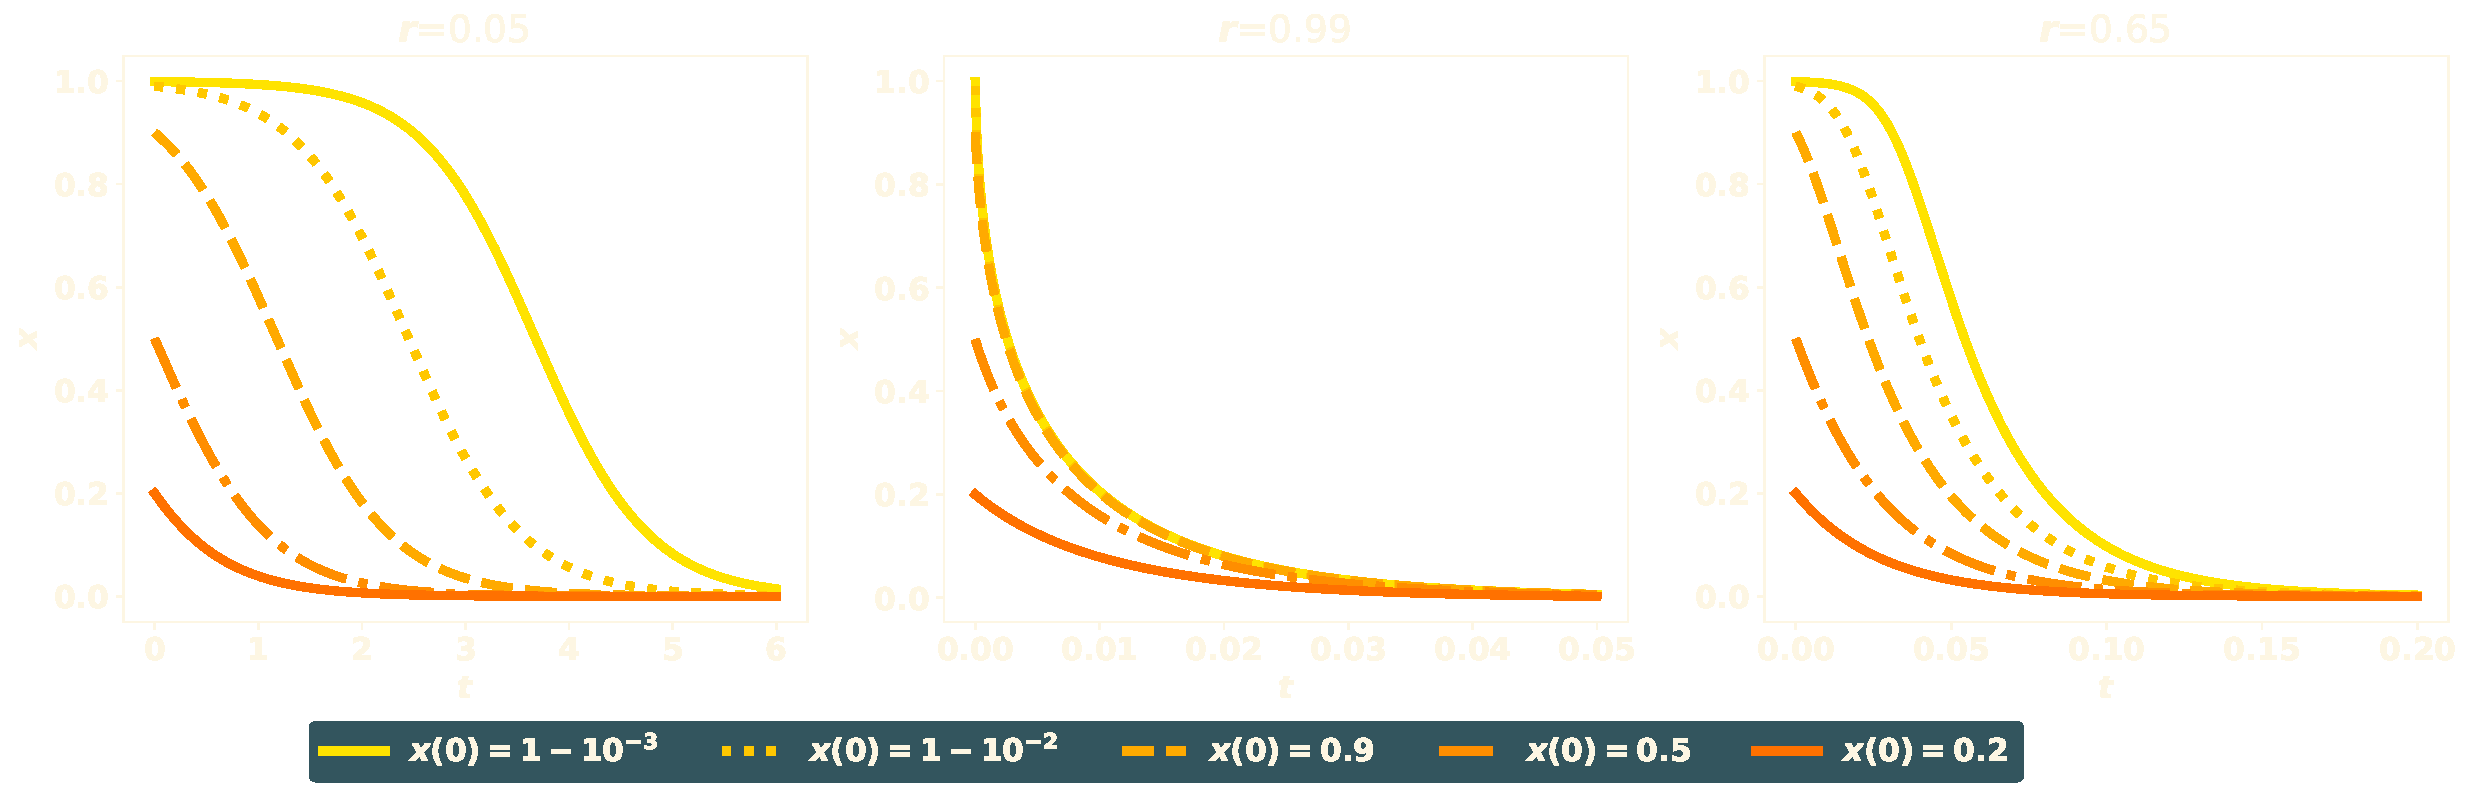
\includegraphics[width=\textwidth]{static/numeric_one.pdf}
\end{frame}

\begin{frame}
    \centering
    
\includegraphics[width=.15\textwidth]{static/1F4B5c.pdf} \hspace{1cm}
    
\includegraphics[width=.15\textwidth]{static/1F4C4.pdf} \hspace{1cm}
    
\includegraphics[width=.15\textwidth]{static/1F4DA.pdf}
\end{frame}

\begin{frame}
    \centering
    \footnotesize
    \begin{theorem}[Disincentive]
    Using the modified utility model, a population of selective poachers is stable
    if and only if:
     \[\frac{r(\theta_r H - F (1 - r)^{\gamma + \beta + \alpha -1})}{(1 - r)^{\alpha}} < \Gamma\]
    \end{theorem}

    \pause
    \vspace{1cm}
    \centering
    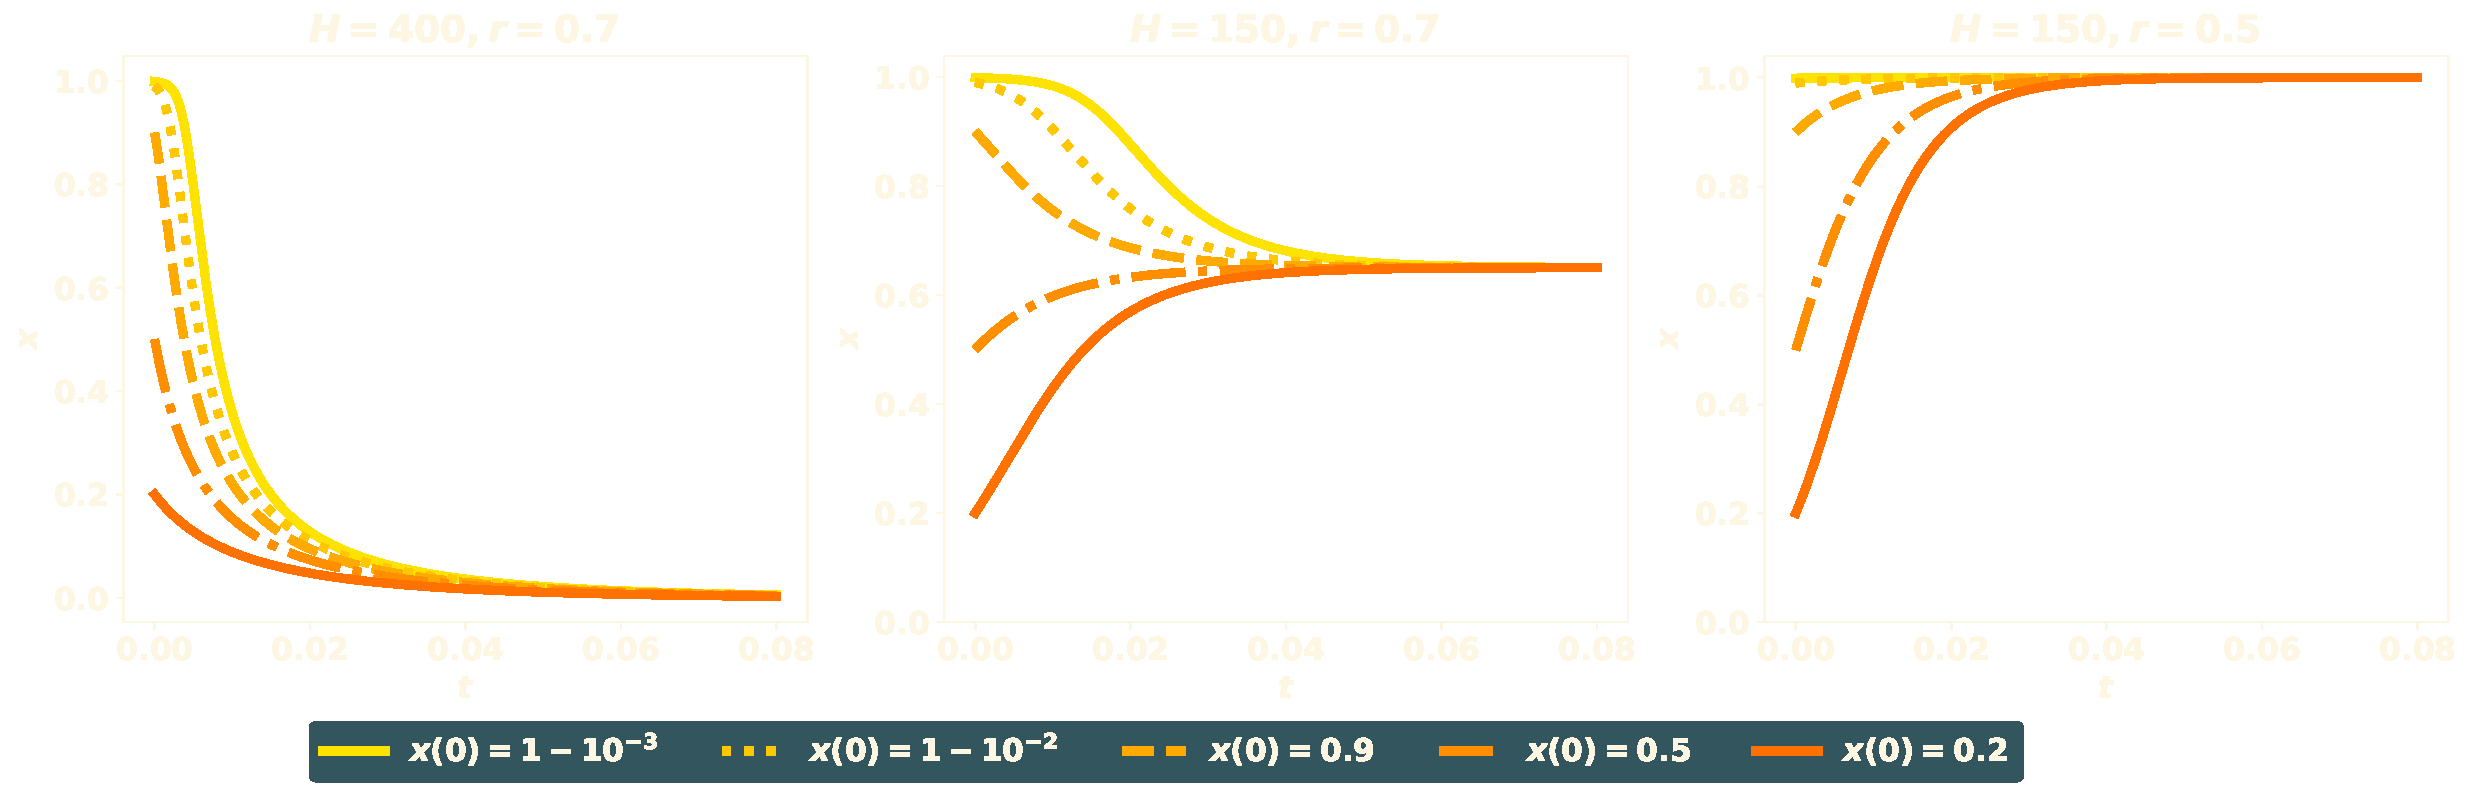
\includegraphics[width=\textwidth]{static/numeric_two.pdf}
\end{frame}

\begin{frame}[fragile]
	\begin{minted}
    [
    framesep=4mm,
    baselinestretch=1.2,
    bgcolor=DarkGray,
    fontsize=\footnotesize,
    ]
    {python}
>>> import numpy as np
>>> from scipy.integrate import odeint
    \end{minted}
\end{frame}

\begin{frame}[fragile]
\textcolor{orange}{
    \resizebox{11cm}{!}{
    \begin{tabular}{lrrrrrrrrrrrrr}
        \toprule
        {} &  $r$ &  $\theta_r$ & $H$ & $F$ &  $\gamma$ &  $\alpha$ & $\beta$ & 
        indiscriminate &  selective &  mixed &  indiscriminate ESS &
        selective ESS &  mixed ESS \\
        \midrule
0 &  0.556 &      0.0 &  0.000 &  0.667 &    0.0 &  0.667 &  0.000 & True &             False &           NaN &                       True &                False &              False \\
1 &  0.242 &      0.0 &  0.500 &  0.000 &    1.0 &  0.500 &  0.000 & True &             False &           NaN &                       True &                False &              False \\
2 &  0.879 &      0.0 &  1.000 &  1.000 &    0.0 &  0.333 &  0.333 & True &             False &           NaN &                       True &                False &              False \\
3 &  0.758 &      0.0 &  0.667 &  1.000 &    0.0 &  0.333 &  1.000 & True &             False &           NaN &                       True &                False &              False \\
4 &  0.788 &      0.0 &  0.250 &  0.000 &    1.0 &  0.250 &  1.000 & True &             False &           NaN &                       True &                False &              False \\
        \bottomrule
        \end{tabular}}}
\end{frame}
\begin{frame}
    \begin{center}
    \vspace{-1cm}

    \includestandalone[width=.8\textwidth]{static/future_work}
    \vspace{1cm}

    \textbf{\textcolor{orange}{
	\small{@NikoletaGlyn}\\
    \small{https://github.com/Nikoleta-v3}\\
    \small{https://arxiv.org/abs/1712.07640}}}
	\end{center}
\end{frame}

\end{document}

